\documentclass[border=5mm]{standalone}
\usepackage{twemojis} 
\usepackage{pgfplots}

\usepgfplotslibrary{colormaps}
\usepgfplotslibrary{patchplots}
\pgfplotsset{
	compat=1.16,
	colormap={mycolormap}{color=(darkgray) color=(lightgray)}
}
\begin{document}

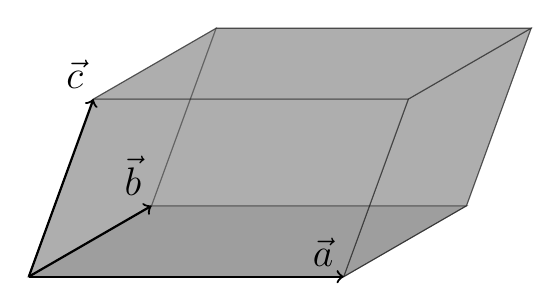
\begin{tikzpicture}

	\begin{scope}[
		x={(4cm,0cm)},
		y={({cos(30)*1.8cm},{sin(30)*1.8cm})},
		z={({cos(70)*2.4cm},{sin(70)*2.4cm})}
		]
		\draw[black,fill=gray,opacity=0.4] (0,0,0) -- (0,0,1) -- (0,1,1) -- (0,1,0) -- cycle;
		\draw[black,fill=gray,opacity=0.6] (0,0,0) -- (1,0,0) -- (1,1,0) -- (0,1,0) -- cycle;
		\draw[black,fill=gray,opacity=0.4] (0,1,0) -- (1,1,0) -- (1,1,1) -- (0,1,1) -- cycle;
		\draw[black,fill=gray,opacity=0.4] (1,0,0) -- (1,0,1) -- (1,1,1) -- (1,1,0) -- cycle;
		\draw[black,fill=gray,opacity=0.4] (0,0,1) -- (1,0,1) -- (1,1,1) -- (0,1,1) -- cycle;
		\draw[black,fill=gray,opacity=0.4] (0,0,0) -- (1,0,0) -- (1,0,1) -- (0,0,1) -- cycle;

		\draw[black,thick,->] (0,0,0) -- (1,0,0) node[above left] {\Large $\vec a$};
		\draw[black,thick,->] (0,0,0) -- (0,1,0) node[above left] {\Large $\vec b$};
		\draw[black,thick,->] (0,0,0) -- (0,0,1) node[above left] {\Large $\vec c$};
	\end{scope}

\end{tikzpicture}
\end{document}
